\subsection{General Overview}

Each team can choose an arbitrary payload to be placed in the rocket. The team decided to develop long-term a set of gliders that are, once deployed from the rocket, flying back to the ground in formation.

For this year, the team prepared a technology demonstrator consisting of only one glider deployed at apogee. This can be extrapolated for a fleet of 7 gliders. The challenge of building more gliders lies in fitting them into a constrained space in the rocket, and still equip them with advanced instrumentation for navigation and control.

\paragraph{Motivation for choosing this payload}
\hfill \break
Rovers such as Curiosity or Spirit have studied Martian terrain and sent back scientific data which may answer questions regarding the origin of life. However, in-situ atmospheric measurements of Mars on longer distances are missing. In order to solve this need, gliders, balloons, or powered planes should overfly Mars and land in areas where rovers cannot. Several projects are proposed by NASA in these directions such as the Preliminary Research Aerodynamic Design to Land on Mars (Prandtl-m) Airplane which aims to be released from a 3U CubeSat and do a 1-hour descent onto the surface of Mars \cite{mars}.

Inspired by the Prandtl-m project, our team aimed to design and build an autonomous glider for the Spaceport America Cup competition, and learn more about the flight dynamics and control of such a complex system.

\begin{table}[h!]
\centering
\begin{tabular}{|p{0.9\columnwidth}|}
\hline
    The payload shall weight 8.8 lb (3.9 kg). \\ \hline
    The payload shall consist of a glider and ballast.  \\ \hline
    The glider shall be deployed at apogee. \\ \hline
    The glider shall deploy its wings passively once ejected from the rocket. \\ \hline
    The glider shall be equipped with an RTK (Real Time Kinematic) GPS used for navigation. \\ \hline
    The glider shall be equipped with a Commercial-Off-The-Shelve autopilot and a pitot tube \\ \hline
    The glider's battery life shall be 1.5 hours. \\ \hline
\end{tabular}
\caption{Top Level Requirements for the payload}
\label{table:se_topLevelR}
\end{table}


\subsection{Design and Manufacturing of one glider}
%Pictures from report here

Due to space constraints, the glider was chosen to be a flying wing with the wings folded in front. XFLR simulations with different airfoils, wing span, wing sweep were performed until the acceptable flight parameters were obtained. The final airfoil is a MH45, with improved (3\%) reflex.

The plane parameters are presented in Table \ref{plane_param}, while the optimal flight parameters are shown in Table \ref{flight_param}.


\begin{table}[h!]
\centering
\begin{tabular}{|l|l|l|}
\hline
\textbf{wing span}      & 0.72 {[}m{]}        & 2.36 {[}ft{]}        \\ \hline
\textbf{wing area}      & 0.07 {[}m$^2${]}    & 0.75 {[}ft$^2${]}   \\ \hline
\textbf{mass}           & 0.27 {[}kg{]}       & 0.61 {[}lb{]}        \\ \hline
\textbf{wing load}      & 4.06 {[}kg/m$^2${]} & 0.83 {[}lb/ft$^2${]} \\ \hline
\textbf{root chord}     & 0.11 {[}m{]}        & 0.36 {[}in{]}        \\ \hline
\textbf{neutral point}  & 0.09 {[}m{]}        & 0.29 {[}in{]}        \\ \hline
\textbf{tip twist}      & -4$^\circ$        &                      \\ \hline
\textbf{aspect ratio}   & 7.50                &                      \\ \hline
\textbf{root-tip chord} & 21$^\circ$        &                      \\ \hline
\end{tabular}
\caption{Plane parameters}
\label{plane_param}
\end{table}



\begin{table}[h!]
\centering
\begin{tabular}{|l|l|}
\hline
\textbf{speed}                    & 18.42 {[}m/s{]} \\ \hline
\textbf{angle-of-attack}          & 4.5$^\circ$                        \\ \hline
\textbf{lift coefficient ($C_L$)} & 0.21                               \\ \hline
\textbf{drag coefficient ($C_D$)} & 0.02                               \\ \hline
\textbf{$C_L$/$C_D$}              & 10                                 \\ \hline
\end{tabular}
\caption{Flight parameters}
\label{flight_param}
\end{table}


The glider was designed in Solidworks. All the components of the glider are encapsulated either in the fuselage, or in the wings, as it can be seen in Figure \ref{f:fuseg} and Figure  \ref{f:wings}.

\begin{figure}[h!]
    \centering
        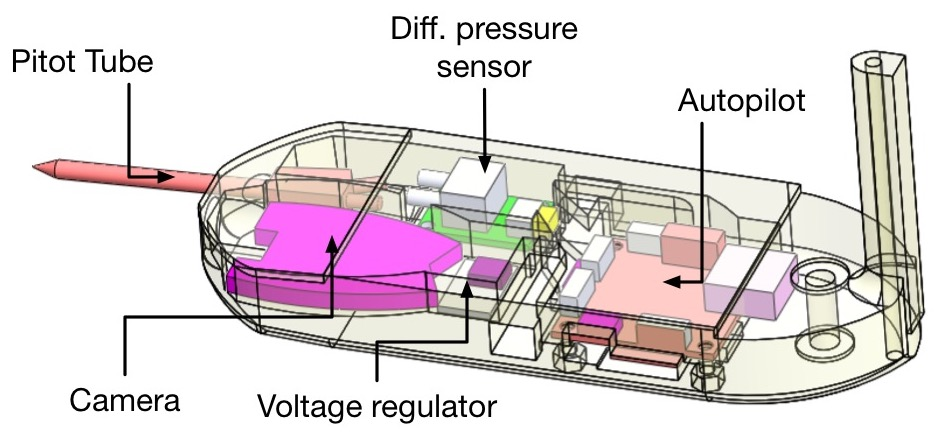
\includegraphics[width=0.5\textwidth]{img/fuselage.jpg}
        \caption{Fuselage with components encapsulated}
        \label{f:fuseg}
 \end{figure}

\begin{figure}[h!]
    \centering
        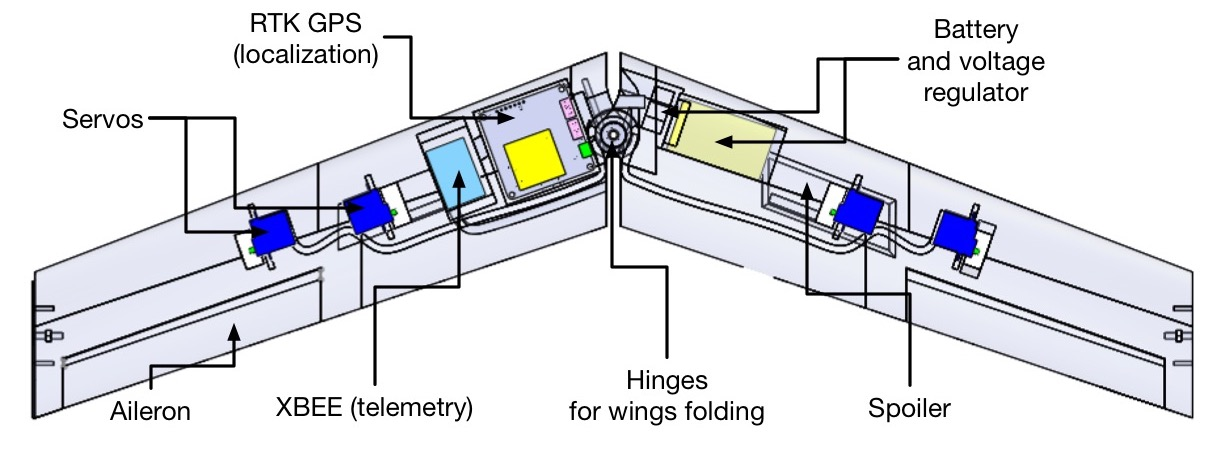
\includegraphics[width=0.5\textwidth]{img/wings.jpg}
        \caption{Wings with components encapsulated}
        \label{f:wings}
 \end{figure}



The wings are folded in front, as it can be seen in Figure \ref{f:folding}.The folding mechanism is made using a torsion spring. The keep-unfolded is obtained using magnets. As the force of the springs is higher than the friction force of the glider's wings inside the box, no additional system to keep the wings folded was requested. The wings are placed one on top of each other, a decision taken in order to optimize the space in the cuboid as soon as possible and to add simplicity in design and manufacturing.

\begin{figure}[h!]
    \centering
        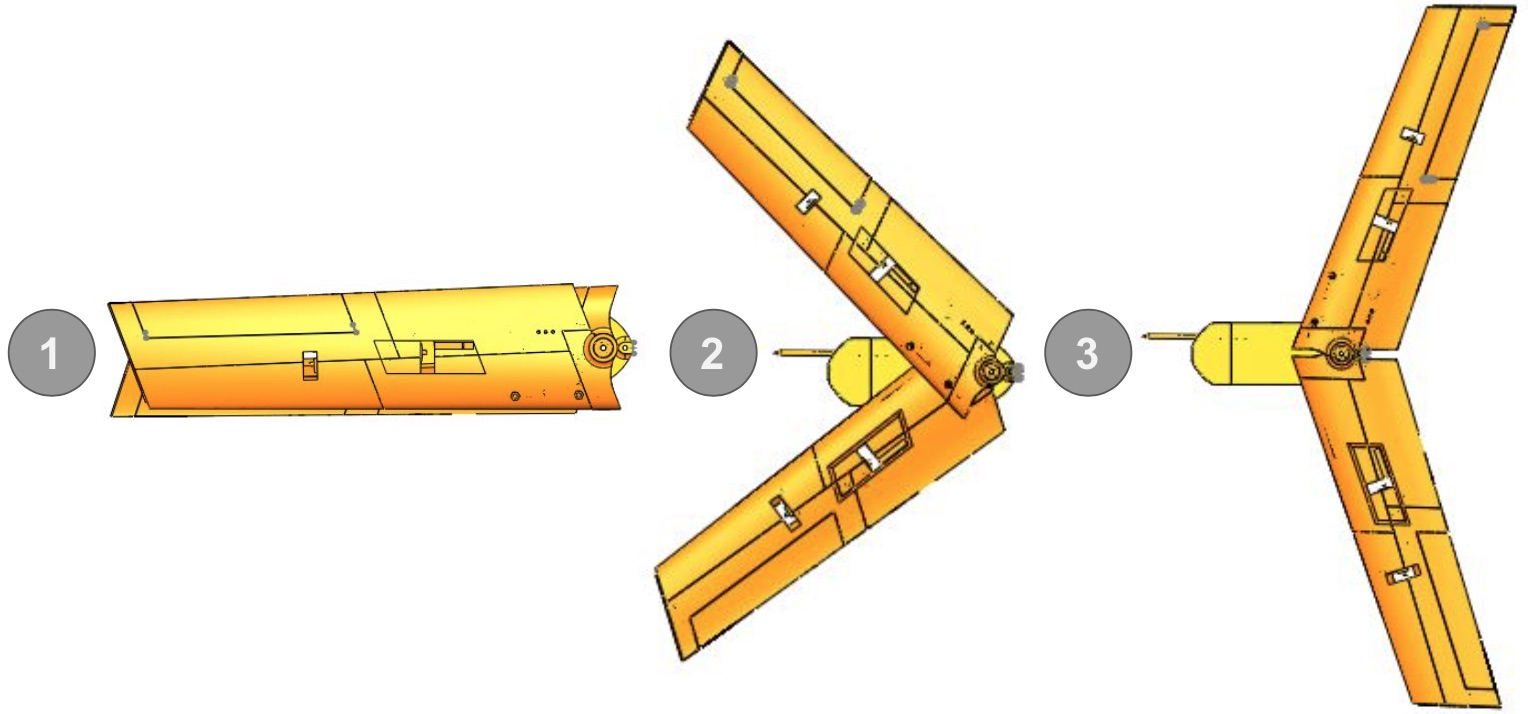
\includegraphics[width=0.5\textwidth]{img/folding.jpg}
        \caption{Unfolding steps 1. The glider is fully folded in its bay. 2. The glider is ejected from the rocket and starts unfolding. 3. The glider is unfolded and starts flying back to the ground}
        \label{f:folding}
 \end{figure}

The second important part of the payload is the ejection system - the system that pushes the glider outside the rocket.
The ejection system is placed in a 4U Cubesat standard cuboid made out of wood and reinforced with glass fiber. The system consists two rails, pulleys, string, spring and one servomotor for locking (Figure \ref{fig:ejection}). The glider is ejected from the rocket by the spring force. The force of the spring is doubled and transmitted to the glider through a strong string. A servomotor keeps the glider in place by injecting a pin into the glider's fuselage block. With this rail-spring system, more gliders can be easily placed in the cuboid in the future.

\begin{figure}[h!]
    \centering
        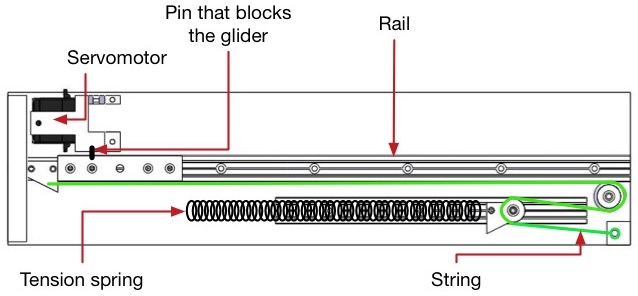
\includegraphics[width=0.5\textwidth]{img/ejection_system.JPG}
        \caption{Ejection System without the glider inside}
        \label{fig:ejection}
 \end{figure}

The glider's wings and fuselage were 3d printed very lightly and reinforced with carbon fibre and glass fibre (where GPS or telemetry antennas were placed). The manufacturing of one of the wings can be seen in Figure \ref{fig:manufact}.

\begin{figure}[h!]
    \centering
        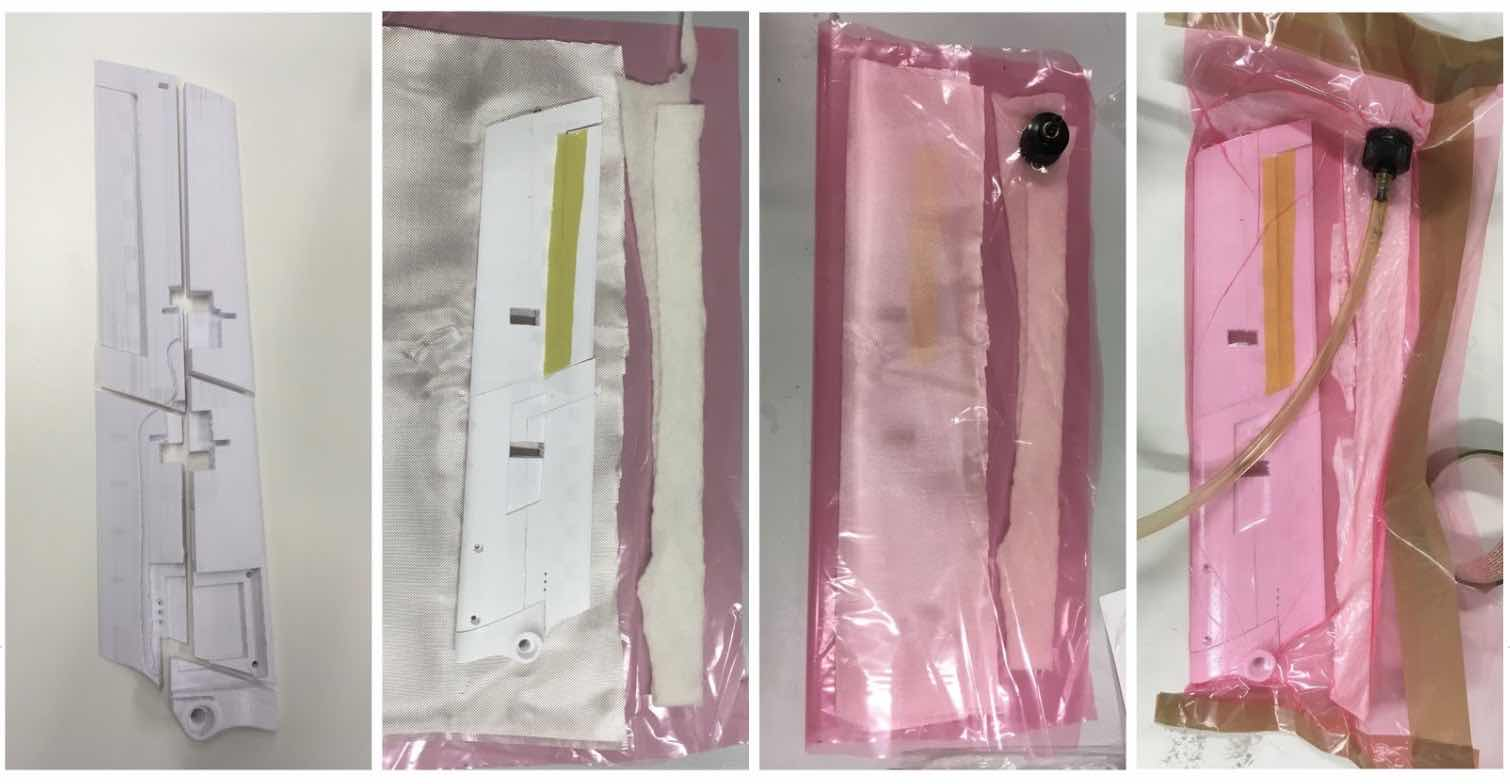
\includegraphics[width=0.5\textwidth]{img/manuf.jpg}
        \caption{Lamination of one of the glider's wings}
        \label{fig:manufact}
 \end{figure}


Figure \ref{fig:final} shows the final design of the wing, as well as the ejection system cuboid.



\begin{figure}[h!]
    \centering
        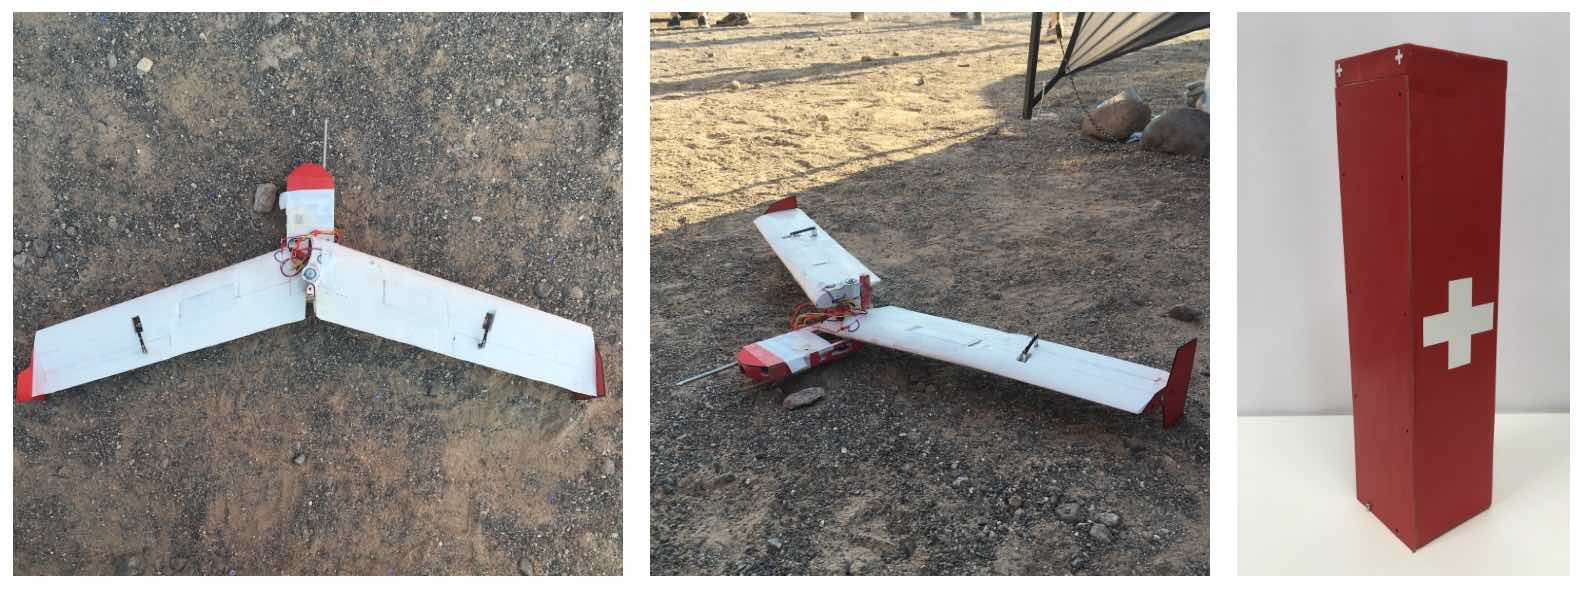
\includegraphics[width=0.5\textwidth]{img/final.jpg}
        \caption{Final design of one glider}
        \label{fig:final}
 \end{figure}

Due to time constraints, this year's glider was not autonomously controlled. Below, the team proposes one navigation concepts that can be put in practice in the future rocket flights.


\subsection{Navigation of the fleet of gliders}
\label{subsection:navcontrol}

Gliders mounted inside a rocket are very challenging to be designed. 
Complex navigation instrumentation cannot be mounted on the gliders, due to space and weight constraints. 
We are thus proposing a solution of using GPS and Ultrawide band beacons for a formation flight of 3 gliders. Both sensors do not require high space and do not weight much.
The concept works as following:
\begin{enumerate}
    \item Ejection Phase: The gliders are ejected from the rocket at apogee
    \item Find Phase: As the gliders might be spread in many directions, it is important to gather them in order to start the formation. For example, the module we propose (DWM1000) has an up to 290 meters communications range. Therefore, for this phase, GPS will be used to determine the position. Once the position is determined for all the 3 gliders, a leader is decided to be the glider closest to the other two. The leader will be thus followed by the other two.
    \item Formation Phase: Once they are close to each other, the UWB beacons are used. They will measure the time of flight, thus the distance between each glider. The idea is to keep a constant distance between the leader and the other two gliders. The orientation of the formation is unknown. For this, we propose to use the barometer to keep a formation parallel to the ground. 
    \item Landing Phase: The landing shall be done in a net, to avoid crashing.
\end{enumerate}


%IR (Impulse Radio) UWB communication systems are based on the transmission of very short duration pulses, which originate very high bandwidth signals. The short duration of the pulses allows a high level of accuracy in time of arrival estimation and as a result a centimeter-level resolution in distance estimation (ranging).

% \label{subsection:navcontrol}

% \paragraph{Navigation using RTK GPS}
% \hfill \break




%Ultrawide beacons 
%Formation
%Check for alternative options, instead of GPS

